\section{Sliding window protocol}\label{sec:sliding-window}
In \autoref{subsec:data-format} it was decided that the format of timestamps would be an integer from 0-255, where 0 to 20 would be considered as newer timestamps than 235 to 255.
However, if all the timestamps from 0 to 20 were lost, there would not be any updates until it has iterated through all other timestamps and back to 0.
To find a better solution to this problem the sliding window protocol was researched.
\\\\
Sliding window protocols are often used where reliable data is required.
This protocol uses window sized buffer space, where the window is a fixed number and the sender will send this number of the packets or bytes to the receiver \cite{design-and-validation-of-computer-protocols}.
Whenever the sender has sent the same number of packets or bytes as the size of the window, it waits for acknowledgements that the receiver has received the packets or bytes before sending additional ones.
Each packet or byte gets a sequence number and the acknowledgement that is sent back also contains the sequence number.
By doing this the receiver can keep track of the packets, remove duplicates, identify missing packets and know which order is the correct one.
\\\\
On \autoref{fig:sliding-window} there is an illustration of a sliding window, where the window size is three packets.
In the first frame, three packets are sent to the receiver, in the second frame the receiver has acknowledged all three packets, but the first acknowledgement fails.
The sliding window for the receiver has moved, but as the sender has only received acknowledgements from the second and third packet, it is unable to move its window and instead sends the first packet again in the third frame.
In the fourth frame, the first packet has been acknowledged, and therefore the sliding window is moved for the sender and the sender is now able to send new packets.
\begin{figure}[H]
    \centering
    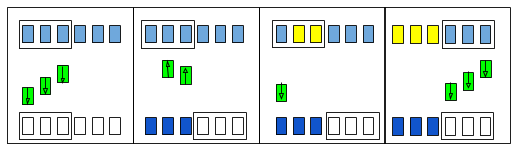
\includegraphics[width=\linewidth]{sliding-window-illustration.png}
    \caption{Sliding window protocol illustration where the top is the sender and the bottom is the receiver.}
    \label{fig:sliding-window}
\end{figure}
\noindent
Reliable data for packets related to goal zones and goal score is important for this project, however the reliability of player positions are not important.
With the \texttt{Sliding Window} protocol a player position would be re-transmitted if it previously failed, and this position would then be outdated because the player might have moved since then.
This means that a sliding window protocol could be used for the game critical aspects transmitted over a UDP connection, such as packets for goal zones and goal scores.
